  \documentclass[msc,numbers,hidelinks]{coppe}

%Added by @MyKo101, code provided by @GerbrichFerdinands
\newlength{\cslhangindent}
\setlength{\cslhangindent}{1.5em}
\newenvironment{cslreferences}%
  {\setlength{\parindent}{0pt}%
  \everypar{\setlength{\hangindent}{\cslhangindent}}\ignorespaces}%
  {\par}

\usepackage{amsmath,amssymb}
\usepackage{hyperref}
\usepackage{longtable}
\usepackage{booktabs}

\providecommand{\tightlist}{%
  \setlength{\itemsep}{0pt}\setlength{\parskip}{0pt}}

\makelosymbols
\makeloabbreviations

\usepackage{color}
\usepackage{fancyvrb}
\newcommand{\VerbBar}{|}
\newcommand{\VERB}{\Verb[commandchars=\\\{\}]}
\DefineVerbatimEnvironment{Highlighting}{Verbatim}{commandchars=\\\{\}}
% Add ',fontsize=\small' for more characters per line
\usepackage{framed}
\definecolor{shadecolor}{RGB}{248,248,248}
\newenvironment{Shaded}{\begin{snugshade}}{\end{snugshade}}
\newcommand{\AlertTok}[1]{\textcolor[rgb]{0.94,0.16,0.16}{#1}}
\newcommand{\AnnotationTok}[1]{\textcolor[rgb]{0.56,0.35,0.01}{\textbf{\textit{#1}}}}
\newcommand{\AttributeTok}[1]{\textcolor[rgb]{0.77,0.63,0.00}{#1}}
\newcommand{\BaseNTok}[1]{\textcolor[rgb]{0.00,0.00,0.81}{#1}}
\newcommand{\BuiltInTok}[1]{#1}
\newcommand{\CharTok}[1]{\textcolor[rgb]{0.31,0.60,0.02}{#1}}
\newcommand{\CommentTok}[1]{\textcolor[rgb]{0.56,0.35,0.01}{\textit{#1}}}
\newcommand{\CommentVarTok}[1]{\textcolor[rgb]{0.56,0.35,0.01}{\textbf{\textit{#1}}}}
\newcommand{\ConstantTok}[1]{\textcolor[rgb]{0.00,0.00,0.00}{#1}}
\newcommand{\ControlFlowTok}[1]{\textcolor[rgb]{0.13,0.29,0.53}{\textbf{#1}}}
\newcommand{\DataTypeTok}[1]{\textcolor[rgb]{0.13,0.29,0.53}{#1}}
\newcommand{\DecValTok}[1]{\textcolor[rgb]{0.00,0.00,0.81}{#1}}
\newcommand{\DocumentationTok}[1]{\textcolor[rgb]{0.56,0.35,0.01}{\textbf{\textit{#1}}}}
\newcommand{\ErrorTok}[1]{\textcolor[rgb]{0.64,0.00,0.00}{\textbf{#1}}}
\newcommand{\ExtensionTok}[1]{#1}
\newcommand{\FloatTok}[1]{\textcolor[rgb]{0.00,0.00,0.81}{#1}}
\newcommand{\FunctionTok}[1]{\textcolor[rgb]{0.00,0.00,0.00}{#1}}
\newcommand{\ImportTok}[1]{#1}
\newcommand{\InformationTok}[1]{\textcolor[rgb]{0.56,0.35,0.01}{\textbf{\textit{#1}}}}
\newcommand{\KeywordTok}[1]{\textcolor[rgb]{0.13,0.29,0.53}{\textbf{#1}}}
\newcommand{\NormalTok}[1]{#1}
\newcommand{\OperatorTok}[1]{\textcolor[rgb]{0.81,0.36,0.00}{\textbf{#1}}}
\newcommand{\OtherTok}[1]{\textcolor[rgb]{0.56,0.35,0.01}{#1}}
\newcommand{\PreprocessorTok}[1]{\textcolor[rgb]{0.56,0.35,0.01}{\textit{#1}}}
\newcommand{\RegionMarkerTok}[1]{#1}
\newcommand{\SpecialCharTok}[1]{\textcolor[rgb]{0.00,0.00,0.00}{#1}}
\newcommand{\SpecialStringTok}[1]{\textcolor[rgb]{0.31,0.60,0.02}{#1}}
\newcommand{\StringTok}[1]{\textcolor[rgb]{0.31,0.60,0.02}{#1}}
\newcommand{\VariableTok}[1]{\textcolor[rgb]{0.00,0.00,0.00}{#1}}
\newcommand{\VerbatimStringTok}[1]{\textcolor[rgb]{0.31,0.60,0.02}{#1}}
\newcommand{\WarningTok}[1]{\textcolor[rgb]{0.56,0.35,0.01}{\textbf{\textit{#1}}}}
\begin{document}

  \title{Titulo de Tese}
  \foreigntitle{Thesis' Title}
    \author{Jefferson}{T. Silvério}
      \advisor{Prof.}{Gisele}{A. Oda}{D.Sc.}
    \advisor{Prof.}{Verónica}{Valentinuzzi}{Ph.D}
    \advisor{Prof.}{Patricia}{Tachinardi}{Ph.D}
  

    \examiner{Prof.}{Nome Completo do Primeiro Examinador}{D.Sc.}
    \examiner{Prof.}{Nome Completo do Segundo Examinador}{Ph.D}
    \examiner{Prof.}{Nome Completo do Terceiro Examinador}{Ph.D}
    \department{IB}
  \date{03}{2021}
    \keyword{Primeira palavra-chave}
    \keyword{Segunda palavra-chave}
    
  % Adiciona Pagina de Titulo
  \maketitle

  % Adiciona Pagina de Rosto com 
  \frontmatter
  
  %Adiciona dedicatorias
  \dedication{A alguém cujo valor é digno desta dedicatória.}
    \chapter*{Agradecimentos}
  Gostaria de agradecer a X
  
  % Adiciona Abstracts
  \begin{abstract}
  ABSTRACT
  \end{abstract}
  \pagebreak
  \begin{foreignabstract}
  ABSTRACT INGLES
  \end{foreignabstract}
  % Adiciona Sumário
  \tableofcontents
  
  % Adiciona Lista de Figuras
    \listoffigures
  
  % Adiciona Lista de Tabelas
    \listoftables
  
  % Adiciona Lista de Simbolos e Abreviacoes
  \printlosymbols
  \printloabbreviations

  % Adiciona Corpo da Tese
  \mainmatter
  \hypertarget{introduuxe7uxe3o-geral}{%
  \chapter*{Introdução Geral}\label{introduuxe7uxe3o-geral}}
  \addcontentsline{toc}{chapter}{Introdução Geral}

  Welcome to the \emph{R Markdown} thesis template. This template is based on (and in many places copied directly from) the Reed College LaTeX template, but hopefully it will provide a nicer interface for those that have never used TeX or LaTeX before. Using \emph{R Markdown} will also allow you to easily keep track of your analyses in \textbf{R} chunks of code, with the resulting plots and output included as well. The hope is this \emph{R Markdown} template gets you in the habit of doing reproducible research, which benefits you long-term as a researcher, but also will greatly help anyone that is trying to reproduce or build onto your results down the road.

  Hopefully, you won't have much of a learning period to go through and you will reap the benefits of a nicely formatted thesis. The use of LaTeX in combination with \emph{Markdown} is more consistent than the output of a word processor, much less prone to corruption or crashing, and the resulting file is smaller than a Word file. While you may have never had problems using Word in the past, your thesis is likely going to be about twice as large and complex as anything you've written before, taxing Word's capabilities. After working with \emph{Markdown} and \textbf{R} together for a few weeks, we are confident this will be your reporting style of choice going forward.

  \textbf{Why use it?}

  \emph{R Markdown} creates a simple and straightforward way to interface with the beauty of LaTeX. Packages have been written in \textbf{R} to work directly with LaTeX to produce nicely formatting tables and paragraphs. In addition to creating a user friendly interface to LaTeX, \emph{R Markdown} also allows you to read in your data, to analyze it and to visualize it using \textbf{R} functions, and also to provide the documentation and commentary on the results of your project. Further, it allows for \textbf{R} results to be passed inline to the commentary of your results. You'll see more on this later.

  \textbf{Who should use it?}

  Anyone who needs to use data analysis, math, tables, a lot of figures, complex cross-references, or who just cares about the final appearance of their document should use \emph{R Markdown}. Of particular use should be anyone in the sciences, but the user-friendly nature of \emph{Markdown} and its ability to keep track of and easily include figures, automatically generate a table of contents, index, references, table of figures, etc. should make it of great benefit to nearly anyone writing a thesis project.

  \textbf{For additional help with bookdown}
  Please visit \href{https://bookdown.org/yihui/bookdown/}{the free online bookdown reference guide}.

  \hypertarget{chronobiology-in-the-wild-toolkit-to-study-daily-rhythms-in-free-living-animals}{%
  \chapter{Chronobiology in the wild: toolkit to study daily rhythms in free-living animals}\label{chronobiology-in-the-wild-toolkit-to-study-daily-rhythms-in-free-living-animals}}

  \emph{Jefferson T. Silvério, Patricia Tachinardi}

  ~

  \emph{Published in Sleep Science - Volume 13, Supplement 2. 2020.}

  ~

  Since chronobiology's foundation has been laid out in the 60s, tremendous progress has been made regarding our knowledge about the nature of the circadian clock, its molecular bases and its synchronization by photic and non-photic stimuli. The majority of these studies have been done in laboratory settings, which, although important, lack information about the adaptive value, ecological significance and plasticity of the biological rhythms in the wild. This concern has been raised several times, along with the development of the field. Methodological difficulties have been the biggest challenges of field studies. However, the recent development of new techniques is opening a wide range of opportunities to investigate biological rhythms in free-ranging animals. In this review, we promote an ecological approach to biological clocks and highlight some methods and newer technologies that can be used to study biological clocks in the wild, along with some examples.

  ~

  \emph{\emph{Keywords:} biological rhythms; wild-clocks; field and laboratory; biologger; free-ranging; activity patterns.}

  \hypertarget{introduction}{%
  \section{Introduction}\label{introduction}}

  Endogenous circadian clocks enable animals to anticipate changes in physiology and behavior to the daily changes in the environment synchronizing their internal state with the 24-hour environmental cycles. Our knowledge of the function and mechanism of these clocks has grown extensively in different levels of organizations such as molecular, cellular, tissue and organs. Most of the studies of the mechanisms and nature of the clock itself has been done in the laboratory, under controlled conditions (Enright \protect\hyperlink{ref-enrightEcologicalAspectsEndogenous1970}{1970}; Morgan \protect\hyperlink{ref-morganEcologicalSignificanceBiological2004}{2004}). Using the laboratory approach, several endogenous circadian rhythms were described in a diverse range of organisms, from mammals to birds, insects and the molecular clocks of bacteria. However, the physiology and behavior of a laboratory animal can be unrepresentative of what happens in the field (Calisi and Bentley \protect\hyperlink{ref-calisiLabFieldExperiments2009}{2009}; Willmer, Stone, and Johnston \protect\hyperlink{ref-willmerEnvironmentalPhysiologyAnimals2005}{2005}). Several authors have brought the argument that we know very little about the ecological significance of circadian rhythms (Enright \protect\hyperlink{ref-enrightEcologicalAspectsEndogenous1970}{1970}; Halle and Stenseth \protect\hyperlink{ref-halleActivityPatternsSmall2000}{2000}; Helm et al. \protect\hyperlink{ref-helmTwoSidesCoin2017}{2017}). The central argument is that to understand the adaptive significance of circadian rhythms, the diversity of temporal strategies and how flexible circadian rhythms are, we must turn to ecological studies in free-living animals. To fill this gap, several recent studies on animal chronobiology have been carried out in free-living animals. These studies investigate the interplay between the endogenous circadian pacemaker and the biotic and abiotic stimuli acting on the plasticity of overt daily rhythms. These studies have suggested that biological rhythms in the wild are much more flexible than previously thought (Hut et al. \protect\hyperlink{ref-hutSearchTemporalNiche2012}{2012}).

  The advancement of chronobiological studies in the field has long been challenged by the difficulty of measuring biological rhythms in nature. In the laboratory, locomotor activity and body temperature (Tb) rhythms have been widely used due to ease of measurement and replicability. Commonly, activity is measured by counting running wheel revolutions, by detecting movement with an infrared motion sensor placed above the animal's cage or by implanting a wireless activity sensor in the animal (Blanchong et al. \protect\hyperlink{ref-blanchongNocturnalDiurnalRhythms1999}{1999}). Measurements of Tb, in turn, are more invasive and can require more expensive equipment. Usually, Tb sensors are implanted surgically in the peritoneal cavity of the animal. These sensors can either be loggers, in which the data is stored in the device or transmitters, which send data to receivers outside the animal (Weinert and Waterhouse \protect\hyperlink{ref-weinertDiurnallyChangingEffects1998}{1998}). When studying free-living animals, however, many of these commonly used methods to study locomotor activity and Tb rhythms are very difficult or simply impossible to be deployed, being it because of technical or financial drawbacks.

  Recent technological advances, such as the miniaturization of sensors and logging devices, have opened a wide variety of opportunities to study biological rhythms in free-living animals. In this mini-review, we will discuss some of the methods being used to assess behavioral and physiological rhythms of free-living animals in both populational and individual levels. We will focus on methods used in the research of terrestrial mammals, although many of them can also be deployed to other taxa and to aquatic and flying animals (Dominoni et al. \protect\hyperlink{ref-dominoniMethodsFieldChronobiology2017}{2017}). It is important to note that most methods require handling the animal for implanting or externally attaching a device. Thus, researchers should always take into account any possible effects this manipulation can have on the animals and on the data obtained (Chmura, Glass, and Williams \protect\hyperlink{ref-chmuraBiologgingPhysiologicalEcological2018}{2018}).

  \hypertarget{chronobiological-studies-in-free-living-animals}{%
  \section{Chronobiological studies in free-living animals}\label{chronobiological-studies-in-free-living-animals}}

  \hypertarget{populational-rhythms}{%
  \subsection{Populational Rhythms}\label{populational-rhythms}}

  Most of the early investigations of clocks in the wild have been carried out focusing on populational rhythms, using observational and trapping methods (Daan and Slopsema \protect\hyperlink{ref-daanShorttermRhythmsForaging1978}{1978}; Halle and Stenseth \protect\hyperlink{ref-halleActivityPatternsSmall2000}{2000}; Kenagy \protect\hyperlink{ref-kenagyPeriodicityDailyActivity1976}{1976}). Using live-traps to infer activity rhythms can be done setting a grid of traps in the study site and then counting the number of captures for a chosen time interval. For example, using hourly record of vole (\emph{Microtus arvalis}) trappings in the wild it was possible to record the pattern of daily activity in these species and their ultradian components (Gerkema and Daan \protect\hyperlink{ref-gerkemaUltradianRhythmsBehavior1985}{1985}). If a higher temporal resolution is required, it is possible to combine live-trapping and direct observations to record the exact time the animals were trapped. Using this approach it was shown that Kangaroo rats (genus Dipodomys) display seasonal change in their start and end time of activity, which might be related to the length changes of sunset (Kenagy \protect\hyperlink{ref-kenagyPeriodicityDailyActivity1976}{1976}). Both observational and live-trapping methods are limited in the range of habitats and diversity of animals they can be applied to. Observational studies have to be done in diurnal species living in open habitats, otherwise, it becomes unfeasible to observe the study species. Small nocturnal animals and animals living in habitats with dense vegetation are not well suited for this technique. On the other hand, trapping studies face the problems of how easily individuals of the study species can be trapped (Halle and Stenseth \protect\hyperlink{ref-halleActivityPatternsSmall2000}{2000}). Both of the above mentioned examples were done in species that are relatively easy to capture in live traps. Kangaroo rats, for example, do not exhibit an aversion to the traps and manipulation. Voles, in turn, leave recognizable tracks aboveground that can guide trap placement and increase trapping success.

  More recently, the use of time-stamped camera-trap images has expanded the study of population activity rhythms to species that cannot be easily observed or captured (Frey et al. \protect\hyperlink{ref-freyInvestigatingAnimalActivity2017}{2017}; Rowcliffe et al. \protect\hyperlink{ref-rowcliffeQuantifyingLevelsAnimal2014}{2014}). Moreover, this non-invasive technique can be used to simultaneously monitor several species that occur in the same area. For example, Mendes and colleagues (Mendes et al. \protect\hyperlink{ref-mendesLandscapeHumanFear2020}{2020}) did an extensive camera-trap study to evaluate the changes in daily activity rhythms of 17 rainforest-dwelling mammal species in response to human disturbance. They found out that there was a shift in the timing of activity in highly disturbed areas, with some species becoming more nocturnal and others more diurnal. Species that were susceptible to preying or hunting were more likely to show activity time shifts. Possible drawbacks of using camera-traps are camera placement bias, detectability of the animals in the camera and the assumption that all individuals of the population will display peak activity at the same time (Frey et al. \protect\hyperlink{ref-freyInvestigatingAnimalActivity2017}{2017}; Rowcliffe et al. \protect\hyperlink{ref-rowcliffeQuantifyingLevelsAnimal2014}{2014}).

  \hypertarget{individual-behavioral-rhythms}{%
  \subsection{Individual behavioral rhythms}\label{individual-behavioral-rhythms}}

  In general, to study individual daily activity patterns it is necessary to continuously follow and record movement and behavior of the same individual for many days (Daan \protect\hyperlink{ref-daanAdaptiveDailyStrategies1981}{1981}), which can be very challenging in the field. Individual monitoring can be done using direct observations (Everts et al. \protect\hyperlink{ref-evertsSeasonalVariationDaily2004}{2004}; Tomotani \protect\hyperlink{ref-tomotaniPosefeitosSincronizacaoEm2011}{2011}), but this method restricts the monitoring of the animal to the times when it is visible. For continuous measurements, it is usually required to attach a device to the animal. Among the earliest measurements of individual activity rhythms using animal-borne devices were those using radio telemetry (Ables \protect\hyperlink{ref-ablesActivityStudiesRed1969}{1969}; Hut, van Oort, and Daan \protect\hyperlink{ref-hutNaturalEntrainmentDawn1999}{1999}). When using this technique, the animal is equipped with a radio telemetry collar that continuously transmits a pulse in a certain radiofrequency that can be picked up by a radio receiver tuned to the same frequency. This way it is possible to locate the animal in the field during defined time intervals. Daily activity patterns are inferred by the size of spatial displacements between these time points throughout day and night. Due to the availability of small and lightweight transmitters, this technique can be used on mammals of nearly any size (Naef-Daenzer \protect\hyperlink{ref-naef-daenzerMiniaturizationEvaluationAttachment2005}{2005}). Telemetry studies are often done manually, thus being very labor-intense and time-consuming. There are automated telemetry systems, which are a feasible alternative to measure activity patterns, as long as the technical and financial requirements to set up the system can be met and errors due to small body size and large home ranges are taken into account (Kays et al. \protect\hyperlink{ref-kaysTrackingAnimalLocation2011}{2011}). Another method that can be used to assess activity patterns based on animal movement are satellite trackers, which previously could only be used in large-sized animals, but are currently being miniaturized (Wikelski and Cooke \protect\hyperlink{ref-wikelskiConservationPhysiology2006}{2006}). An important advantage of this technique is that data can be obtained remotely, with no need to locate the animal after the tag is deployed.

  Individual-level rhythms can also be measured with newer biologging devices, which are attached to the animal's body and can record onboard physiological and behavioral parameters including activity, Tb, heart rate and skin humidity (Ropert-Coudert and Wilson \protect\hyperlink{ref-ropert-coudertTrendsPerspectivesAnimalattached2005}{2005}; Rutz and Hays \protect\hyperlink{ref-rutzNewFrontiersBiologging2009}{2009}). Given the advancements in the biologging technologies, devices are now smaller and capable of recording multiple parameters in a frequency of hundreds of points per second, providing insight into the details of the animal's life (Ropert-Coudert and Wilson \protect\hyperlink{ref-ropert-coudertTrendsPerspectivesAnimalattached2005}{2005}). Due to the onboard memory, the main drawback of biologgers is the need to recapture the animals to obtain the data.

  Examples of biologging devices used to monitor animal behavior in chronobiological studies include lightloggers and accelerometers. Lightloggers are devices that were originally designed to be used in geolocation in bird migration studies but are particularly interesting for chronobiology. Lightloggers are being used to conduct research on a number of small rodents, recording their temporal patterns of exposure to light. Studies that are benefitted by the use of lightloggers include research on diurnal animals that retreat to nests, subterranean or semi-fossorial animals and hibernating animals in which exposure to light means the animals are active above ground. Accelerometers, in turn, are tri-axial devices that continuously record fine-scale movement. The data generated by accelerometers can be used to quantify gross activity timing, identify behaviors based on movement patterns, quantify time-activity budgets and indirectly derive energy expenditure (Brown et al. \protect\hyperlink{ref-brownObservingUnwatchableAcceleration2013}{2013}; Ropert-Coudert and Wilson \protect\hyperlink{ref-ropert-coudertTrendsPerspectivesAnimalattached2005}{2005}; Rutz and Hays \protect\hyperlink{ref-rutzNewFrontiersBiologging2009}{2009}).

  Lightloggers were used to investigate the daily and seasonal patterns of activity in wild red squirrels (\emph{Tamiasciurus hudsonicus}) and arctic ground squirrels (\emph{Urocitellus parryii}) (Williams et al. \protect\hyperlink{ref-williamsLightLoggersReveal2014}{2014}). Using these devices, they could calculate the total time outside of the nest, the number of activity bouts per day, time of the first emergence in the morning and return to nest at night. They showed that the level of activity was flexible and correlated with changes in the thermoregulatory conditions of the environment. On a different rodent species, the tuco-tuco (genus Ctenomys), a combination of lightloggers and accelerometry was used to investigate the activity patterns of a subterranean rodent in outdoor enclosures (Jannetti et al. \protect\hyperlink{ref-jannettiDayNightSubterranean2019}{2019}). In this study, accelerometers were used to record gross motor activity while lightloggers recorded time on surface. A combination of both methods, therefore, could discriminate levels of aboveground activity and below-ground activity when the animal is inside its burrow system. The study showed that time of day and temperature were the main environmental conditions modulating time spent on the surface (Jannetti et al. \protect\hyperlink{ref-jannettiDayNightSubterranean2019}{2019}) and that there was a shift from diurnal to nocturnal levels of activity when the same animals were transferred from outdoor enclosure to controlled laboratory conditions (Jannetti et al. \protect\hyperlink{ref-jannettiDayNightSubterranean2019}{2019}; Tachinardi et al. \protect\hyperlink{ref-tachinardiNocturnalDiurnalSwitches2015}{2015}). Although this study was done in outdoor enclosures, this approach can also be used in free-ranging animals. Shifts in the timing of activity are also known to happen in other species of rodents besides \emph{Ctenomys sp.} (Hut et al. \protect\hyperlink{ref-hutSearchTemporalNiche2012}{2012}; Kronfeld-Schor et al. \protect\hyperlink{ref-kronfeld-schorChronobiologyInterspecificInteractions2017}{2017}) and are among the most dramatic discrepancies between rhythms in the field and lab. Biologgers are a helpful addition to approach this phenomenon at the individual level and boost this investigation. The examples provided here highlight possible scenarios where the use of biologging devices can be used to reveal the intimacy and complexity of rhythms in the wild, investigating chronobiological questions and the flexibility of circadian and seasonal rhythms.

  Other alternative technologies can be used to assess rhythms in the wild, such as RFID (Radio Frequency Identification) and newly developed ones such as the BATS system. RFID are small tags that can be used to identify individuals in a population Passive RFID tags do not require their battery to operate and are powered by the energy from the reader's radio waves. They are largely used to identify farm and laboratory animals, being very small and attached either externally or subcutaneously. RFID tags can be used to record activity rhythms by placing readers in locations that the animals visit regularly, such as nests or feeders. This setup allows the recording of the rhythmicity of visits to a specific location where the reader is placed (Vinne et al. \protect\hyperlink{ref-vinneMaximisingSurvivalShifting2019}{2019}). Although this technique is usually deployed in outdoor enclosures it could be used in free-living animals that have fixed nests or feeding locations. The BATS system is an interesting technology that is fully automated (Duda et al. \protect\hyperlink{ref-dudaBATSAdaptiveUltra2018}{2018}; S. P. Ripperger, Carter, Page, et al. \protect\hyperlink{ref-rippergerThinkingSmallNextgeneration2019}{2019}). It is composed of small lightweight proximity sensors and a set of receiver stations that are distributed in the study site. The proximity sensors can record interactions between two animals in a sampling rate of seconds and then transmit these data to the base stations. This system can also be used to derive movement trajectory even in structurally complex habitats (S. P. Ripperger, Carter, Page, et al. \protect\hyperlink{ref-rippergerThinkingSmallNextgeneration2019}{2019}). Ripperger and colleagues have used this system to study the behavioral ecology of bats, such as the mother-offspring interactions in noctule bats (\emph{Nyctalus noctule}) (Ripperger et al. \protect\hyperlink{ref-rippergerProximitySensorsCommon2019}{2019}) and the social structure of the common vampire bats (\emph{Desmodus rotundus}) (S. P. Ripperger, Carter, Duda, et al. \protect\hyperlink{ref-rippergerVampireBatsThat2019}{2019}). Although the BATS system was developed to investigate a different set of questions it seems to be a great new technology to assist in the study of reproduction, social synchronization and the social influences on biological rhythms.

  \hypertarget{physiological-rhythms}{%
  \subsection{Physiological rhythms}\label{physiological-rhythms}}

  Biologgers can also be used to assess daily rhythms of physiological variables, enabling the investigation of physiological adjustments to the changes in environmental conditions faced by free-living animals. Tb is the physiological variable most studied in wild chronobiology. It is usually measured and recorded by temperature loggers implanted into the abdomen. This method was used to monitor Tb in free-living arctic ground squirrels (\emph{Urocitellus parryii}) throughout the year, showing that in these animals Tb is arrhythmic during hibernation but displays an entrained 24-hour rhythm in the active season even during the weeks of constant sun (Williams et al. \protect\hyperlink{ref-williamsDataLoggingBody2011}{2011}). Monitoring of Tb was also used to record dramatic shifts from diurnally to nocturnality when golden spiny mice (\emph{Acomys russatus}) are transferred from large outdoor enclosures to the laboratory (Levy, Dayan, and Kronfeld-Schor \protect\hyperlink{ref-levyRelationshipGoldenSpiny2007}{2007}). This study is a clear example of how the assessment of physiological rhythms can be important in the investigation of the plasticity of biological rhythms, since the same physiological variable can be measured in both conditions, as opposed to measuring different types of behavioral rhythms under field and laboratory conditions (e.g.~foraging in the field and wheel running in the laboratory).

  In the laboratory, energy expenditure rhythms can be assessed by measuring hourly rates of oxygen consumption using respirometry chambers, for instance, which is not possible in free-living animals. Since heart rate can be a proxy to energy expenditure, it is a valuable physiological variable in chronobiological studies involving energetics. Heart rate sensors can be attached to the skin, implanted subcutaneously (Tøien et al. \protect\hyperlink{ref-toienHibernationBlackBears2011}{2011}) or even placed non-surgically in the reticulum of ruminants (Signer et al. \protect\hyperlink{ref-signerVersatileTelemetrySystem2010}{2010}). These devices can either be loggers (Tøien et al. \protect\hyperlink{ref-toienHibernationBlackBears2011}{2011}) or transmitters (Signer et al. \protect\hyperlink{ref-signerVersatileTelemetrySystem2010}{2010}).

  Brain electrical activity is also of interest to chronobiological studies since it can be used to investigate sleep patterns. Recently, miniature loggers have been developed to measure electrophysiological brain activity (Massot et al. \protect\hyperlink{ref-massotONEIROSNewMiniature2019}{2019}; Vyssotski et al. \protect\hyperlink{ref-vyssotskiMiniatureNeurologgersFlying2006}{2006}). Studies using these loggers have, for instance, provided insights into the ecology of sleep in sloths (Rattenborg et al. \protect\hyperlink{ref-rattenborgSleepingOutsideBox2008}{2008}) and even indicated that birds can sleep during flight (Rattenborg et al. \protect\hyperlink{ref-rattenborgEvidenceThatBirds2016}{2016}).

  \hypertarget{conclusion}{%
  \section{Conclusion}\label{conclusion}}

  In this mini-review, we highlighted some, but not all, methods that can be applied in chronobiological studies in the wild. There is a range of new devices and techniques currently being developed that could be applied to free-living animals to assess biological rhythms. The combination of different devices can also be used to discriminate and investigate how some behaviors or physiology interact, even at the cellular and molecular levels (Jansen et al. \protect\hyperlink{ref-jansenBearCircadianClock2016}{2016}). The fast methodological advancement and the increasing interest of chronobiologists in field studies are key aspects to narrow the gap between what we know about the circadian clocks in the lab and what we know about their functional significance in nature.

  \hypertarget{acknowledgements}{%
  \section{Acknowledgements}\label{acknowledgements}}

  We would like to thank Gisele Oda for the revision and suggestions that improved the manuscript; Danilo Flôres, Milene Jannetti and Giovane Improta for discussion of everything chronobiology; and the organizing committee of the XV Latin American Symposium on Chronobiology. JTS was funded in part by the Coordenação de Aperfeiçoamento de Pessoal de Nível Superior - Brasil (CAPES) - Finance Code 001, CAPES scholarship (88882.377383/2019-01) and additional grant from Fundação de Amparo à Pesquisa do Estado de São Paulo (FAPESP) (2017/19680-2). PT was funded by FAPESP fellowship 2017/22973-1.

  \hypertarget{artigo-tese}{%
  \chapter{Artigo Tese}\label{artigo-tese}}

  \hypertarget{methods}{%
  \section{Methods}\label{methods}}

  \hypertarget{study-site}{%
  \subsection{Study site}\label{study-site}}

  Field work was conducted at one site located approximately 5km away from the village of Anillaco, in the province of La Rioja, northwest of Argentina. The study site (-66.95°, -028.80, 1325m; Fig. \ref{fig:methods-map}) is a relatively undisturbed natural area - with little human disturbance and no artificial light source - surrounded by the Sierra de Velasco moutain range, located within the Monte Desert biome. The Monte Desert is characterized as an open shrubland dominated by Zygophyllaceae (\emph{Larrea cuneifolia} Cav., \emph{Tricomaria usillo}), Fabaceae (\emph{Prosopis torquata}, \emph{Senna aphylla}) and Cactaceae (\emph{Trichocereus} spp, \emph{Tephrocactus} spp) (Abraham et al. \protect\hyperlink{ref-abrahamOverviewGeographyMonte2009}{2009}; Aranda-Rickert, Diez, and Marazzi \protect\hyperlink{ref-aranda-rickertExtrafloralNectarFuels2014}{2014}; Fracchia et al. \protect\hyperlink{ref-fracchiaDispersalArbuscularMycorrhizal2011}{2011}). At the study site a non-extensive survey of the plant community divided in three transects showed a dominance of the families Zygophyllaceae (\emph{Larrea cuneifolia}, \emph{Tricomaria usillo}), Poaceae (\emph{Microchloa indica}, \emph{Aristida mendocina}) and Fabaceae (\emph{Zuccagnia punctata}) (see Appendix). The climate is arid with marked daily cycle and seasonality in temperature and rainfall (see Appendix). The mean annual temperature is 16.6°C (Fracchia et al. \protect\hyperlink{ref-fracchiaDispersalArbuscularMycorrhizal2011}{2011}), with clear differences in the daily range and between summer and winter months (Abraham et al. \protect\hyperlink{ref-abrahamOverviewGeographyMonte2009}{2009}). The mean annual rainfall ranges from 145 to 380mm concentrated almost exclusively in the summer months (Fracchia et al. \protect\hyperlink{ref-fracchiaDispersalArbuscularMycorrhizal2011}{2011}).
  \begin{figure}
  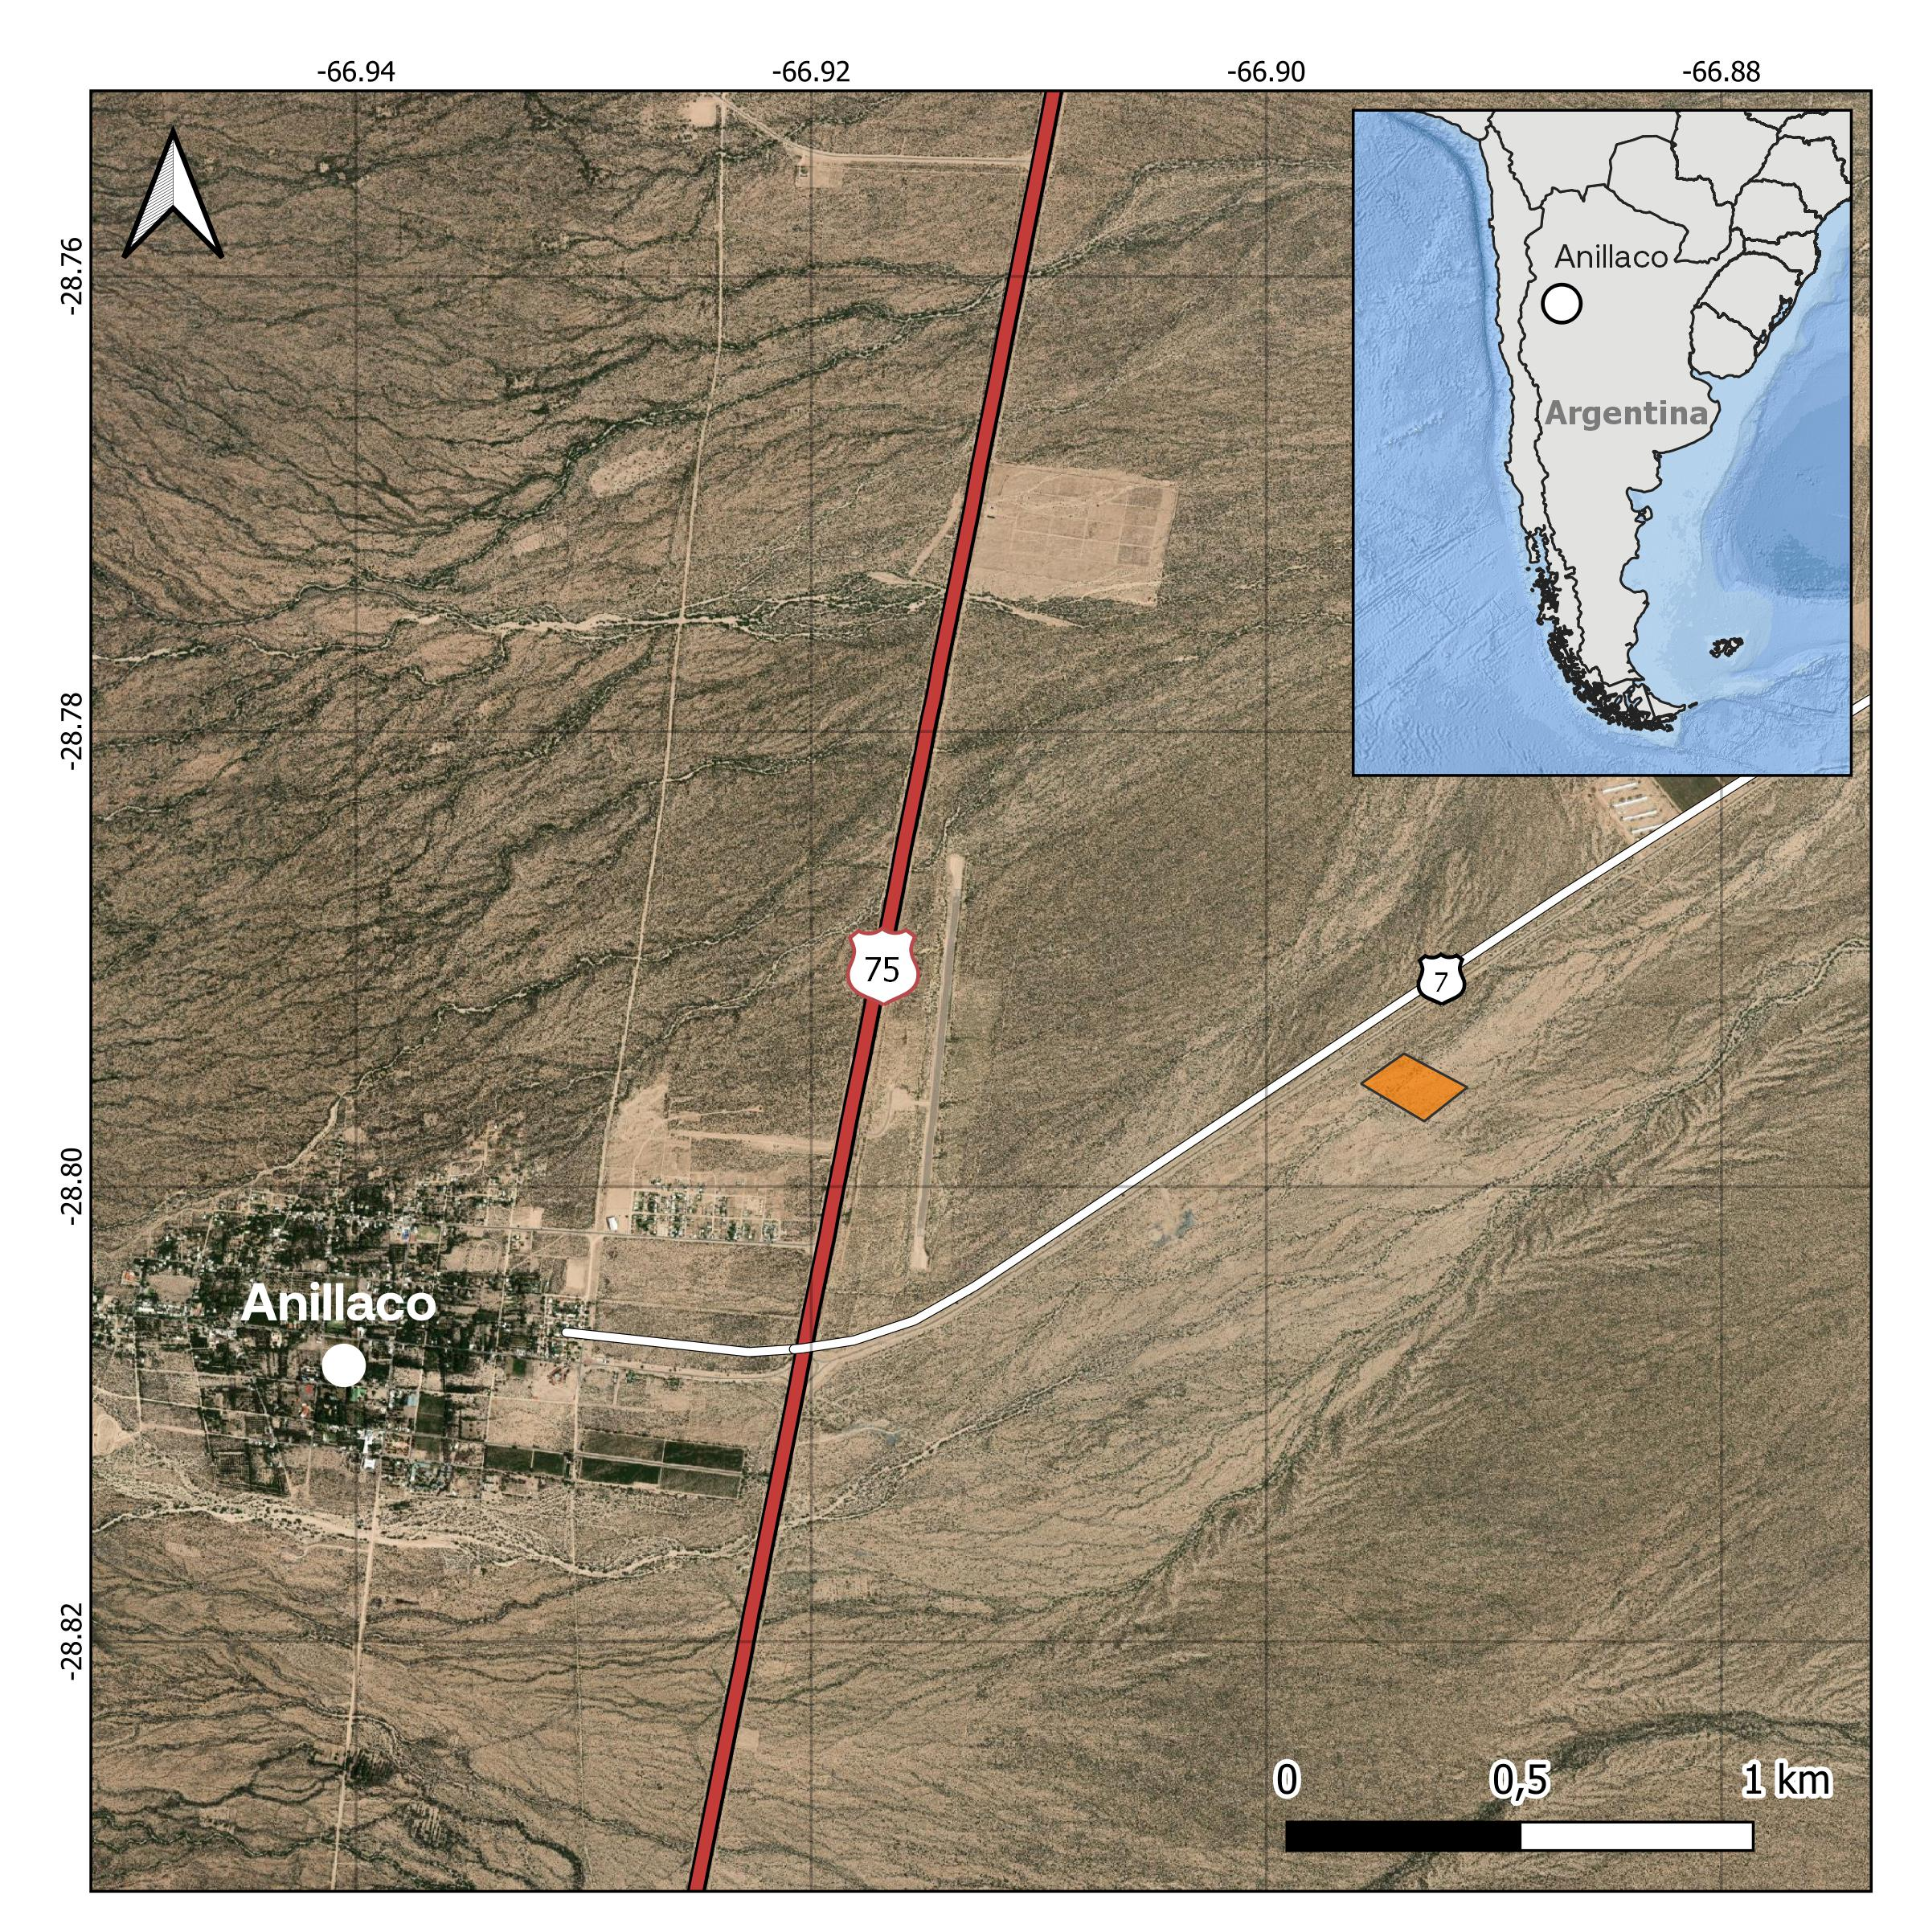
\includegraphics[width=1\linewidth]{../05_figures/map/tuco_map} \caption{Study site location (orange icon) at the Monte Desert, approximately 5km away form the village of Anillaco, northwest of Argentina}\label{fig:methods-map}
  \end{figure}
  \hypertarget{study-species}{%
  \subsection{Study species}\label{study-species}}

  The studied \emph{Ctenomys} population lacks a formal phylogenetic and taxonomic classification but there are some lines of evidence suggesting that the study area is occupied by a single unidentified species (REF Amaya form and function). In other studies this Ctenomys' species has been referred informally as the Anillaco tuco-tuco (REF Amaya) and as \emph{Ctenomys aff. knightii} (REF) or \emph{Ctenomys cf.~knightii} (REF).

  \hypertarget{capture-and-recapture}{%
  \subsection{Capture and Recapture}\label{capture-and-recapture}}

  Tucos were captured by searching the study area for fresh signs of burrow entrances. Once found, custom made traps, similar in functionality to a Shermann trap, were placed at the burrow's entrance. Our custom made traps were made out of PVC tubing (35cm length, 10cm diameter) with a spring-loaded aluminum door at one and a cul-de-sac at the other. The traps were placed in the field during the morning and checked every hour until the beginning of the night, when they were taken out.

  After being captured, adult tucos (\textgreater120g) were first anesthetized in order to be carefully examined and receive a collar with activity sensors. We used a clear plastic anesthesia chamber (volume?) with a clip-on lid and a cotton ball inside. We added approximately 0.5 mL of isoflurane (REF) to the cotton ball before transferring the animal from the trap to the plastic anesthesia chamber. While in the chamber tucos were observed for breathing, blinking and loss of righting reflex. Once the tucos could not right themselves they were removed from the chamber. Out of the chamber anesthetezied animals were weighted, sexed, marked with a subcutaneous identification PIT Tag (Passive Integrative Transponder. Allflex, Brasil) and received a collar with activity sensors and a telemetry transmitter (SOM-2011. Wildlife Materials, Illinois, USA). Tucos were them placed back in the trap and observed until fully recovered. Once recovered tucos were transported and released in the same burrow they were captured. Marked animals were left in the field for 5-10 days before being recaptured. The telemetry transmitter were used to maximize the animals relocation and recapture, avoiding the loss the other devices.

  \hypertarget{activity-data}{%
  \subsection{Activity data}\label{activity-data}}

  The accelerometers attached to the animal's collar were configured to record at a 10 Hz sampling frequency with a 4G sensitivity. The lightloggers were set to record at a sample each 5 minutes with range of sensitivity from 0.3 to 19000 lux.
  The data collection were done The recaptures were done with the to the

  Accelerometers are devices that continuously record the animal's movement in a three axis orthogonal system with a high sampling frequency (REF).
  \begin{itemize}
  \tightlist
  \item
    apendice:
    \begin{itemize}
    \tightlist
    \item
      fotos da armadilha
    \item
      foto do colar
    \end{itemize}
  \end{itemize}
  a lightlogger (Migrate Technology, Cambridge, UK), a accelerometer (Axy3. Technosmart, Rome, Italy)
  \begin{itemize}
  \tightlist
  \item
    acelerometros
  \item
    luximetros
  \item
    radiotelemetria
  \item
    armadilhas
  \item
    permissoes
  \end{itemize}
  \hypertarget{activity-levels}{%
  \subsection{Activity Levels}\label{activity-levels}}

  Vectorial Dynamic Body Acceleration (VeDBA, Qasem et al. \protect\hyperlink{ref-qasemTriAxialDynamicAcceleration2012}{2012}) was used as a proxy for the animal's activity level. VeDBA was calculated by: (i) Estimating the effect of the gravitational force over the accelerometer, also known as static acceleration. The static acceleration can be estimated by applying a moving average over the raw acceleration data. There is not a consensus over the the number of points to calculate the moving average with, which can be dependent on the study species and device's recording frequency (REF??). Generally, a 1 or 2-second moving average is used to calculated the static acceleration (REF??). However, in the case of the tucos we opted to use a 4-second moving average (40 data points) after following the method proposed by (Shepard et al. \protect\hyperlink{ref-shepardDerivationBodyMotion2008}{2008}, see Appendix). (ii) Calculating the acceleration correspondent to the animal's movement, also know as Dynamic Body Acceleration (DBA). The DBA was calculated by subtracting the static acceleration from the raw data. (iii) Lastly, we calculate the VeDBA by the vectorial sum of the DBA over the device's axis, using:

  \[ VeDBA = \sqrt{Xd^2 + Yd^2 + Zd^2} \]

  \hypertarget{conclusuxe3o-geral}{%
  \chapter*{Conclusão Geral}\label{conclusuxe3o-geral}}
  \addcontentsline{toc}{chapter}{Conclusão Geral}

  If we don't want Conclusion to have a chapter number next to it, we can add the \texttt{\{-\}} attribute.

  \appendix

  \appendix

  \hypertarget{appendix}{%
  \chapter*{Appendix}\label{appendix}}
  \addcontentsline{toc}{chapter}{Appendix}

  \hypertarget{anillacos-plant-community}{%
  \chapter{Anillaco's Plant Community}\label{anillacos-plant-community}}

  Following methods similar to Aranda-Rickert, Diez, and Marazzi (\protect\hyperlink{ref-aranda-rickertExtrafloralNectarFuels2014}{2014}) a non-extensive survey of the plant community was done in May 2019. Three perpendicular 50m transects were defined near the study site (COORDINATES). A point-intercept method was used to record plant species present in the transects, species right below the sampling points were registered in the data. Sampling points were defined every 1m along the 50m transects. Plant species were identified in the field by a Botanist, except for a few members of the Poaceae family.

  The results for the plant survey is in line with what has been described in the literature for the region (Abraham et al. \protect\hyperlink{ref-abrahamOverviewGeographyMonte2009}{2009}; Aranda-Rickert, Diez, and Marazzi \protect\hyperlink{ref-aranda-rickertExtrafloralNectarFuels2014}{2014}; Fracchia et al. \protect\hyperlink{ref-fracchiaDispersalArbuscularMycorrhizal2011}{2011}). The results show a dominance of Zygolhyllaceae, Poaceae and Fabaceae families. The relative frequency of plant families and species recorded in the area are shown in the graphs below (Fig. \ref{fig:appendix-plants}).
\begin{Shaded}
\begin{Highlighting}[]
\KeywordTok{include\_graphics}\NormalTok{(}\StringTok{"../05\_figures/plants/plant\_frequency.png"}\NormalTok{)}
\end{Highlighting}
\end{Shaded}
  \begin{figure}
  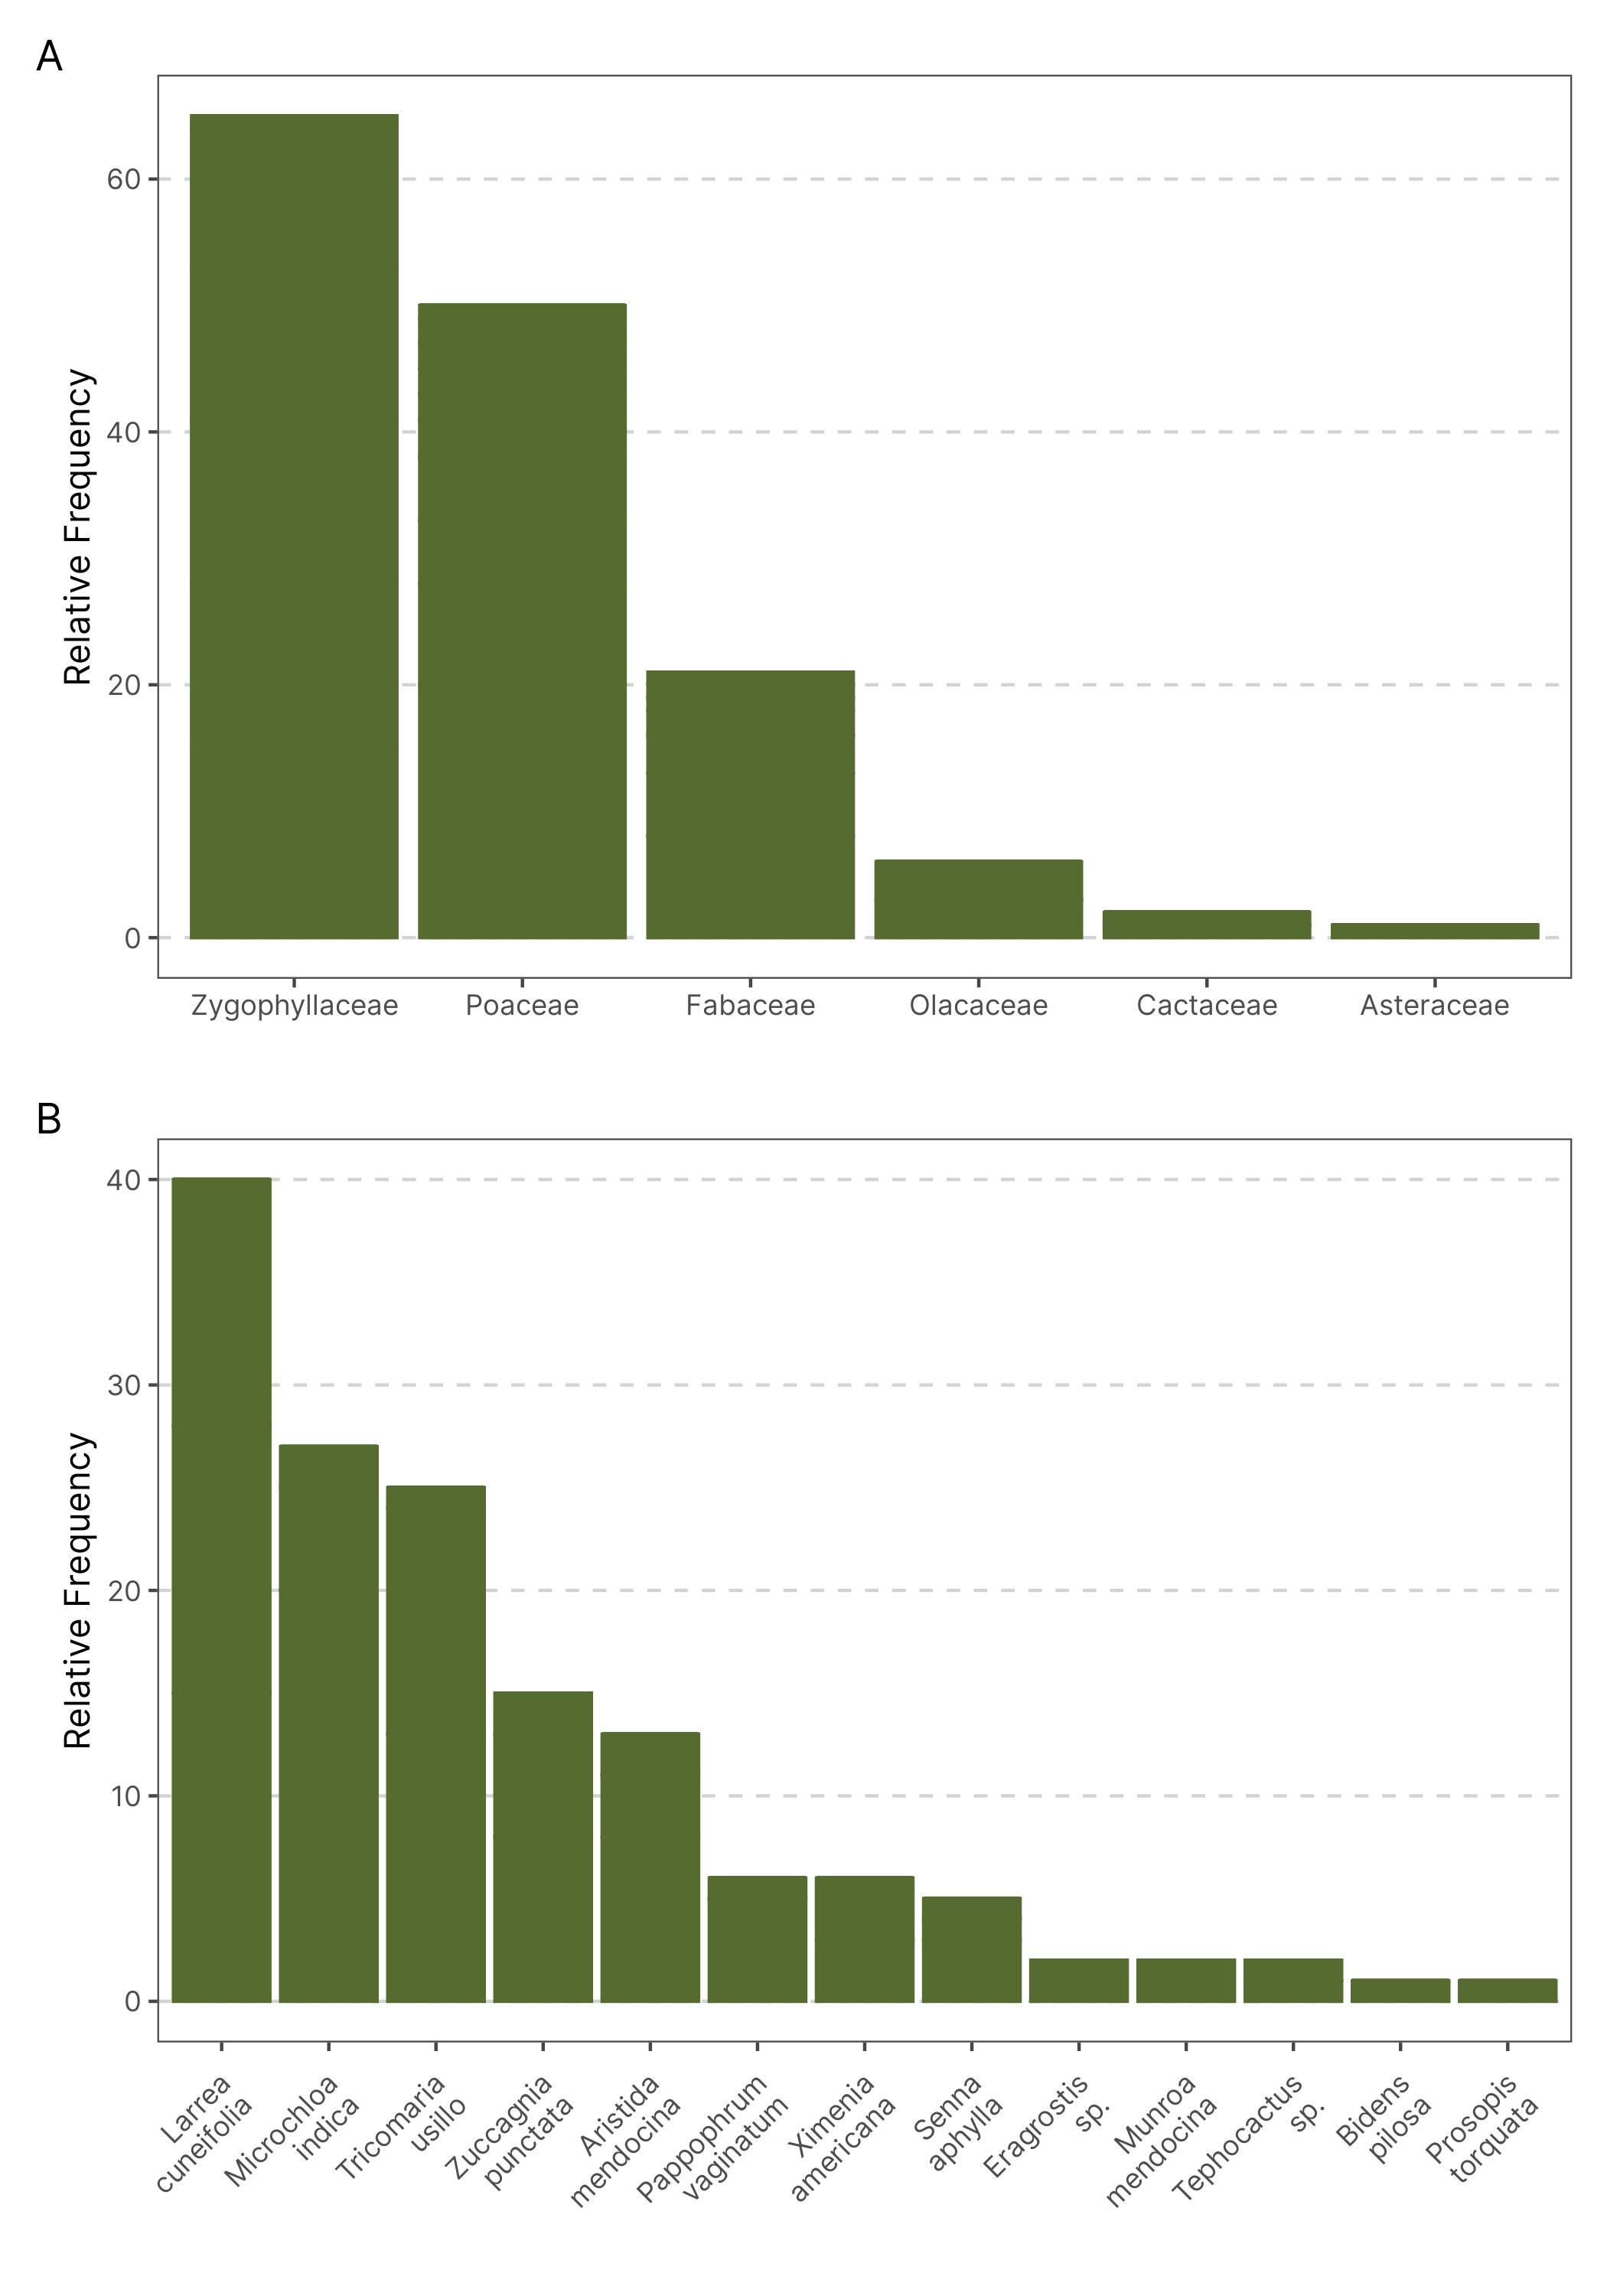
\includegraphics[width=1\linewidth]{../05_figures/plants/plant_frequency} \caption{Relative frequency of plants family (A) and species (B) in three transects near the Study Site. The plant community is dominated by members of the Zygolhyllaceae, Poaceae and Fabaceae families and is in accordance with what has been described in the literature. (n = 145)}\label{fig:appendix-plants}
  \end{figure}
  \hypertarget{anillacos-weather}{%
  \chapter{Anillaco's Weather}\label{anillacos-weather}}
\begin{Shaded}
\begin{Highlighting}[]
\KeywordTok{include\_graphics}\NormalTok{(}\StringTok{"../05\_figures/weather/weather.png"}\NormalTok{)}
\end{Highlighting}
\end{Shaded}
  \begin{figure}
  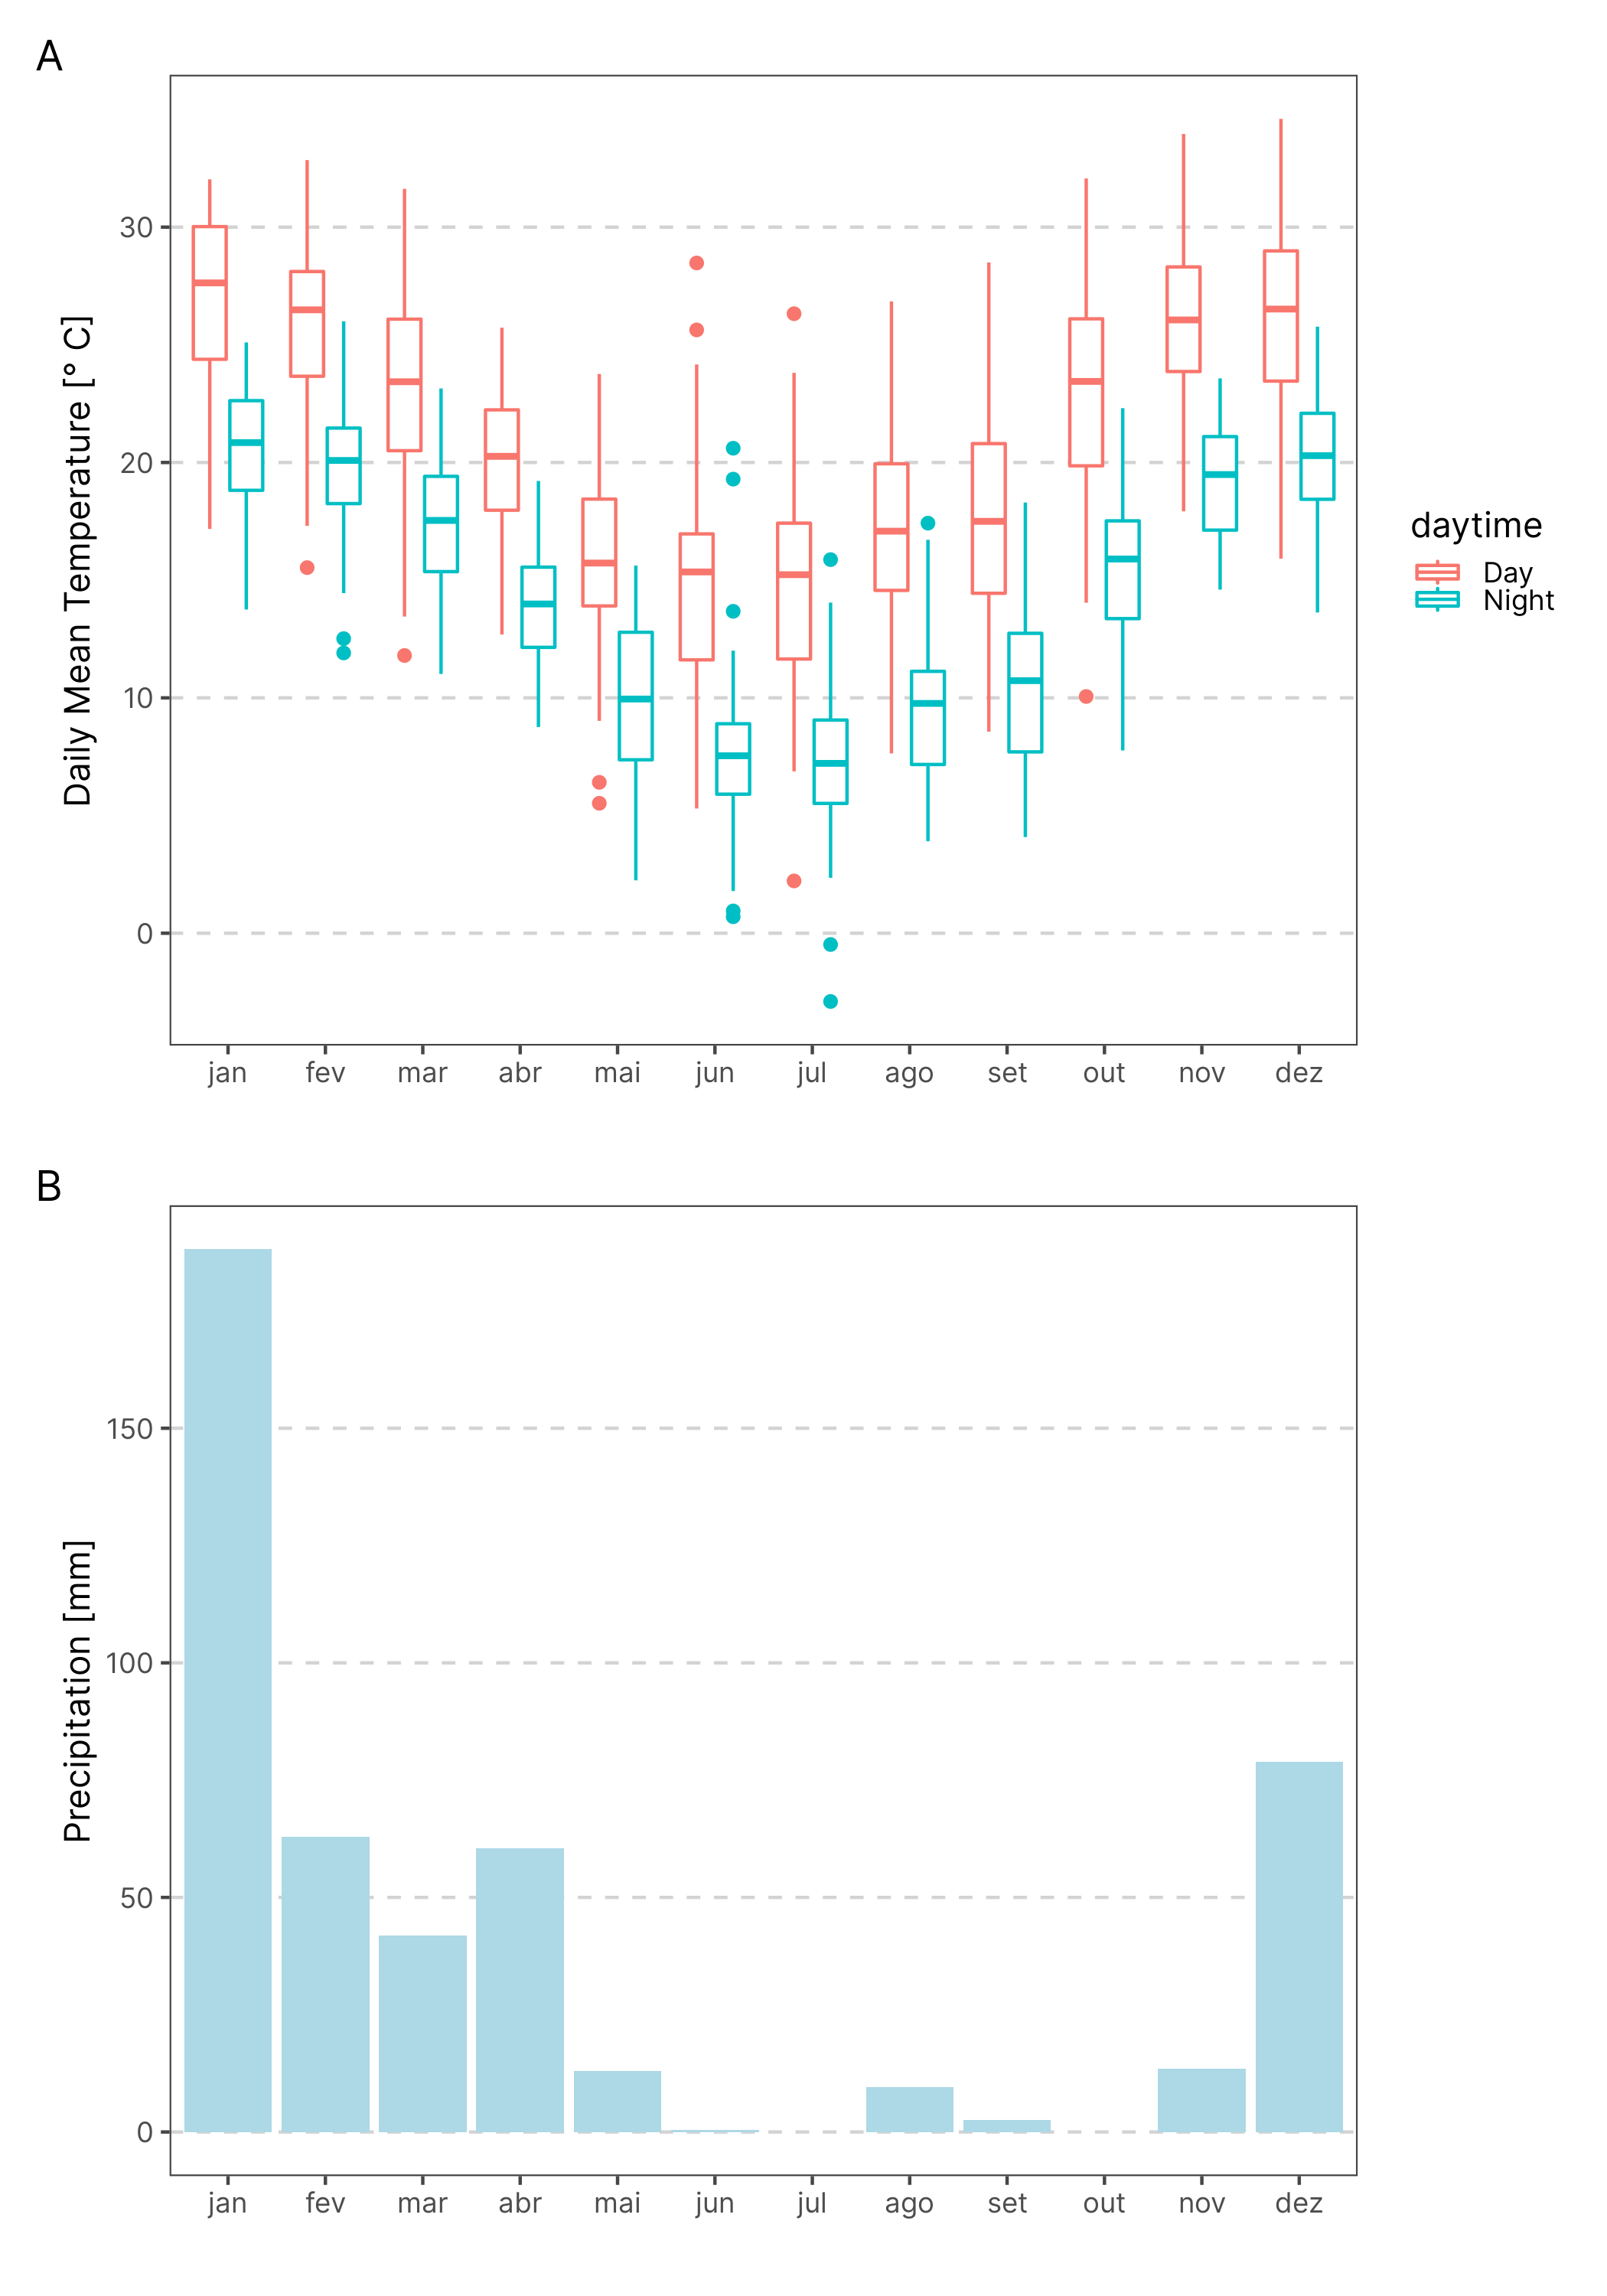
\includegraphics[width=1\linewidth]{../05_figures/weather/weather} \end{figure}

  \backmatter
  \bibliographystyle{$biblio-style$}
  \bibliography{thesis}

  \hypertarget{references}{%
  \chapter*{References}\label{references}}
  \addcontentsline{toc}{chapter}{References}

  \noindent

  \setlength{\parindent}{-0.20in}
  \setlength{\leftskip}{0.20in}
  \setlength{\parskip}{8pt}

  \hypertarget{refs}{}
  \begin{cslreferences}
  \leavevmode\hypertarget{ref-ablesActivityStudiesRed1969}{}%
  Ables, Ernest D. 1969. ``Activity Studies of Red Foxes in Southern Wisconsin.'' \emph{The Journal of Wildlife Management} 33 (1): 145. \url{https://doi.org/10.2307/3799662}.

  \leavevmode\hypertarget{ref-abrahamOverviewGeographyMonte2009}{}%
  Abraham, E., H. F. del Valle, F. Roig, L. Torres, J. O. Ares, F. Coronato, and R. Godagnone. 2009. ``Overview of the Geography of the Monte Desert Biome (Argentina).'' \emph{Journal of Arid Environments} 73 (2): 144--53. \url{https://doi.org/10.1016/j.jaridenv.2008.09.028}.

  \leavevmode\hypertarget{ref-aranda-rickertExtrafloralNectarFuels2014}{}%
  Aranda-Rickert, Adriana, Patricia Diez, and Brigitte Marazzi. 2014. ``Extrafloral Nectar Fuels Ant Life in Deserts.'' \emph{AoB PLANTS} 6 (January). \url{https://doi.org/10.1093/aobpla/plu068}.

  \leavevmode\hypertarget{ref-blanchongNocturnalDiurnalRhythms1999}{}%
  Blanchong, J. A., T. L. McElhinny, M. M. Mahoney, and L. Smale. 1999. ``Nocturnal and Diurnal Rhythms in the Unstriped Nile Rat, Arvicanthis Niloticus.'' \emph{Journal of Biological Rhythms} 14 (5): 364--77. \url{https://doi.org/10.1177/074873099129000777}.

  \leavevmode\hypertarget{ref-brownObservingUnwatchableAcceleration2013}{}%
  Brown, Danielle D., Roland Kays, Martin Wikelski, Rory Wilson, and A. Peter Klimley. 2013. ``Observing the Unwatchable Through Acceleration Logging of Animal Behavior.'' \emph{Animal Biotelemetry} 1 (1): 20. \url{https://doi.org/10.1186/2050-3385-1-20}.

  \leavevmode\hypertarget{ref-calisiLabFieldExperiments2009}{}%
  Calisi, Rebecca M., and George E. Bentley. 2009. ``Lab and Field Experiments: Are They the Same Animal?'' \emph{Hormones and Behavior} 56 (1): 1--10. \url{https://doi.org/10.1016/j.yhbeh.2009.02.010}.

  \leavevmode\hypertarget{ref-chmuraBiologgingPhysiologicalEcological2018}{}%
  Chmura, Helen E., Thomas W. Glass, and Cory T. Williams. 2018. ``Biologging Physiological and Ecological Responses to Climatic Variation: New Tools for the Climate Change Era.'' \emph{Frontiers in Ecology and Evolution} 6 (July): 92. \url{https://doi.org/10.3389/fevo.2018.00092}.

  \leavevmode\hypertarget{ref-daanAdaptiveDailyStrategies1981}{}%
  Daan, Serge. 1981. ``Adaptive Daily Strategies in Behavior.'' In \emph{Handbook of Behavioral Neurobiology}, 4:563. Plenum Press.

  \leavevmode\hypertarget{ref-daanShorttermRhythmsForaging1978}{}%
  Daan, Serge, and Steven Slopsema. 1978. ``Short-Term Rhythms in Foraging Behaviour of the Common Vole,Microtus Arvalis.'' \emph{Journal of Comparative Physiology} 127 (3): 215--27. \url{https://doi.org/10.1007/BF01350112}.

  \leavevmode\hypertarget{ref-dominoniMethodsFieldChronobiology2017}{}%
  Dominoni, Davide M., Susanne Åkesson, Raymond Klaassen, Kamiel Spoelstra, and Martin Bulla. 2017. ``Methods in Field Chronobiology.'' \emph{Philosophical Transactions of the Royal Society B: Biological Sciences} 372 (1734): 20160247. \url{https://doi.org/10.1098/rstb.2016.0247}.

  \leavevmode\hypertarget{ref-dudaBATSAdaptiveUltra2018}{}%
  Duda, Niklas, Thorsten Nowak, Markus Hartmann, Michael Schadhauser, Björn Cassens, Peter Wägemann, Muhammad Nabeel, et al. 2018. ``BATS: Adaptive Ultra Low Power Sensor Network for Animal Tracking.'' Article. \emph{Sensors} 18 (10): 3343. \url{https://doi.org/10.3390/s18103343}.

  \leavevmode\hypertarget{ref-enrightEcologicalAspectsEndogenous1970}{}%
  Enright, J T. 1970. ``Ecological Aspects of Endogenous Rhythmicity.'' \emph{Annual Review of Ecology and Systematics} 1 (1): 221--38. \url{https://doi.org/10.1146/annurev.es.01.110170.001253}.

  \leavevmode\hypertarget{ref-evertsSeasonalVariationDaily2004}{}%
  Everts, Lammina G., Arjen M. Strijkstra, Roelof A. Hut, Ilse E. Hoffmann, and Eva Millesi. 2004. ``Seasonal Variation in Daily Activity Patterns of Free-Ranging European Ground Squirrels (Spermophilus Citellus).'' \emph{Chronobiology International} 21 (1): 57--71. \url{https://doi.org/10.1081/cbi-120027982}.

  \leavevmode\hypertarget{ref-fracchiaDispersalArbuscularMycorrhizal2011}{}%
  Fracchia, S., L. Krapovickas, A. Aranda-Rickert, and V. S. Valentinuzzi. 2011. ``Dispersal of Arbuscular Mycorrhizal Fungi and Dark Septate Endophytes by Ctenomys Cf. Knighti (Rodentia) in the Northern Monte Desert of Argentina.'' \emph{Journal of Arid Environments} 75 (11): 1016--23. \url{https://doi.org/10.1016/j.jaridenv.2011.04.034}.

  \leavevmode\hypertarget{ref-freyInvestigatingAnimalActivity2017}{}%
  Frey, Sandra, Jason T. Fisher, A. Cole Burton, and John P. Volpe. 2017. ``Investigating Animal Activity Patterns and Temporal Niche Partitioning Using Camera-Trap Data: Challenges and Opportunities.'' \emph{Remote Sensing in Ecology and Conservation} 3 (3): 123--32. \url{https://doi.org/10.1002/rse2.60}.

  \leavevmode\hypertarget{ref-gerkemaUltradianRhythmsBehavior1985}{}%
  Gerkema, Menno, and Serge Daan. 1985. ``Ultradian Rhythms in Behavior the Case of the Common Vole (Microtus Arvalis).'' \url{https://doi.org/10.1007/978-3-642-70483-3_3}.

  \leavevmode\hypertarget{ref-halleActivityPatternsSmall2000}{}%
  Halle, S., and Nils Chr Stenseth, eds. 2000. \emph{Activity Patterns in Small Mammals: An Ecological Approach}. Ecological Studies, v. 141. Berlin ; New York: Springer.

  \leavevmode\hypertarget{ref-helmTwoSidesCoin2017}{}%
  Helm, Barbara, Marcel E. Visser, William Schwartz, Noga Kronfeld-Schor, Menno Gerkema, Theunis Piersma, and Guy Bloch. 2017. ``Two Sides of a Coin: Ecological and Chronobiological Perspectives of Timing in the Wild.'' \emph{Philosophical Transactions of the Royal Society B: Biological Sciences} 372 (1734): 20160246. \url{https://doi.org/10.1098/rstb.2016.0246}.

  \leavevmode\hypertarget{ref-hutSearchTemporalNiche2012}{}%
  Hut, Roelof A., Noga Kronfeld-Schor, Vincent van der Vinne, and Horacio De la Iglesia. 2012. ``In Search of a Temporal Niche: Enviromental Factors.'' In \emph{Progress in Brain Research}, 199:281--304. Elsevier. \url{https://doi.org/10.1016/B978-0-444-59427-3.00017-4}.

  \leavevmode\hypertarget{ref-hutNaturalEntrainmentDawn1999}{}%
  Hut, Roelof A., Bob E. H. van Oort, and Serge Daan. 1999. ``Natural Entrainment Without Dawn and Dusk: The Case of the European Ground Squirrel ( \emph{Spermophilus} \emph{Citellus} ).'' \emph{Journal of Biological Rhythms} 14 (4): 290--99. \url{https://doi.org/10.1177/074873099129000704}.

  \leavevmode\hypertarget{ref-jannettiDayNightSubterranean2019}{}%
  Jannetti, Milene G., C. Loren Buck, Veronica S. Valentinuzzi, and Gisele A. Oda. 2019. ``Day and Night in the Subterranean: Measuring Daily Activity Patterns of Subterranean Rodents (Ctenomys Aff. Knighti) Using Bio-Logging.'' \emph{Conservation Physiology} 7 (1). \url{https://doi.org/10.1093/conphys/coz044}.

  \leavevmode\hypertarget{ref-jansenBearCircadianClock2016}{}%
  Jansen, Heiko T., Tanya Leise, Gordon Stenhouse, Karine Pigeon, Wayne Kasworm, Justin Teisberg, Thomas Radandt, Robert Dallmann, Steven Brown, and Charles T. Robbins. 2016. ``The Bear Circadian Clock Doesn't `Sleep' During Winter Dormancy.'' \emph{Frontiers in Zoology} 13 (1): 42. \url{https://doi.org/10.1186/s12983-016-0173-x}.

  \leavevmode\hypertarget{ref-kaysTrackingAnimalLocation2011}{}%
  Kays, Roland, Sameer Tilak, Margaret Crofoot, Tony Fountain, Daniel Obando, Alejandro Ortega, Franz Kuemmeth, et al. 2011. ``Tracking Animal Location and Activity with an Automated Radio Telemetry System in a Tropical Rainforest.'' \emph{The Computer Journal} 54 (12): 1931--48. \url{https://doi.org/10.1093/comjnl/bxr072}.

  \leavevmode\hypertarget{ref-kenagyPeriodicityDailyActivity1976}{}%
  Kenagy, G. J. 1976. ``The Periodicity of Daily Activity and Its Seasonal Changes in Free-Ranging and Captive Kangaroo Rats.'' \emph{Oecologia} 24 (2): 105--40. \url{https://doi.org/10.1007/BF00572754}.

  \leavevmode\hypertarget{ref-kronfeld-schorChronobiologyInterspecificInteractions2017}{}%
  Kronfeld-Schor, Noga, Marcel E. Visser, Lucia Salis, and Jan A. van Gils. 2017. ``Chronobiology of Interspecific Interactions in a Changing World.'' \emph{Philosophical Transactions of the Royal Society B: Biological Sciences} 372 (1734): 20160248. \url{https://doi.org/10.1098/rstb.2016.0248}.

  \leavevmode\hypertarget{ref-levyRelationshipGoldenSpiny2007}{}%
  Levy, Ofir, Tamar Dayan, and Noga Kronfeld-Schor. 2007. ``The Relationship Between the Golden Spiny Mouse Circadian System and Its Diurnal Activity: An Experimental Field Enclosures and Laboratory Study.'' \emph{Chronobiology International} 24 (4): 599--613. \url{https://doi.org/10.1080/07420520701534640}.

  \leavevmode\hypertarget{ref-massotONEIROSNewMiniature2019}{}%
  Massot, Bertrand, Sébastien Arthaud, Baptiste Barrillot, Johanna Roux, Gianina Ungurean, Pierre-Hervé Luppi, Niels C. Rattenborg, and Paul-Antoine Libourel. 2019. ``ONEIROS, a New Miniature Standalone Device for Recording Sleep Electrophysiology, Physiology, Temperatures and Behavior in the Lab and Field.'' \emph{Journal of Neuroscience Methods}, Methods and models in sleep research: A Tribute to Vincenzo Crunelli, 316 (March): 103--16. \url{https://doi.org/10.1016/j.jneumeth.2018.08.030}.

  \leavevmode\hypertarget{ref-mendesLandscapeHumanFear2020}{}%
  Mendes, Calebe P., Daiane Carreira, Felipe Pedrosa, Gabrielle Beca, Laís Lautenschlager, Paula Akkawi, William Bercê, Katia M. P. M. B. Ferraz, and Mauro Galetti. 2020. ``Landscape of Human Fear in Neotropical Rainforest Mammals.'' \emph{Biological Conservation} 241 (January): 108257. \url{https://doi.org/10.1016/j.biocon.2019.108257}.

  \leavevmode\hypertarget{ref-morganEcologicalSignificanceBiological2004}{}%
  Morgan, Elfed. 2004. ``Ecological Significance of Biological Clocks.'' \emph{Biological Rhythm Research} 35 (1-2): 3--12. \url{https://doi.org/10.1080/09291010412331313205}.

  \leavevmode\hypertarget{ref-naef-daenzerMiniaturizationEvaluationAttachment2005}{}%
  Naef-Daenzer, B. 2005. ``Miniaturization (0.2 G) and Evaluation of Attachment Techniques of Telemetry Transmitters.'' \emph{Journal of Experimental Biology} 208 (21): 4063--8. \url{https://doi.org/10.1242/jeb.01870}.

  \leavevmode\hypertarget{ref-qasemTriAxialDynamicAcceleration2012}{}%
  Qasem, Lama, Antonia Cardew, Alexis Wilson, Iwan Griffiths, Lewis G. Halsey, Emily L. C. Shepard, Adrian C. Gleiss, and Rory Wilson. 2012. ``Tri-Axial Dynamic Acceleration as a Proxy for Animal Energy Expenditure; Should We Be Summing Values or Calculating the Vector?'' \emph{PLOS ONE} 7 (2): e31187. \url{https://doi.org/10.1371/journal.pone.0031187}.

  \leavevmode\hypertarget{ref-rattenborgEvidenceThatBirds2016}{}%
  Rattenborg, Niels C., Bryson Voirin, Sebastian M. Cruz, Ryan Tisdale, Giacomo Dell'Omo, Hans-Peter Lipp, Martin Wikelski, and Alexei L. Vyssotski. 2016. ``Evidence That Birds Sleep in Mid-Flight.'' OriginalPaper. \emph{Nature Communications} 7 (1): 1--9. \url{https://doi.org/10.1038/ncomms12468}.

  \leavevmode\hypertarget{ref-rattenborgSleepingOutsideBox2008}{}%
  Rattenborg, Niels C., Bryson Voirin, Alexei L. Vyssotski, Roland W. Kays, Kamiel Spoelstra, Franz Kuemmeth, Wolfgang Heidrich, and Martin Wikelski. 2008. ``Sleeping Outside the Box: Electroencephalographic Measures of Sleep in Sloths Inhabiting a Rainforest.'' \emph{Biology Letters} 4 (4): 402--5. \url{https://doi.org/10.1098/rsbl.2008.0203}.

  \leavevmode\hypertarget{ref-rippergerProximitySensorsCommon2019}{}%
  Ripperger, Simon, Linus Günther, Hanna Wieser, Niklas Duda, Martin Hierold, Björn Cassens, Rüdiger Kapitza, Alexander Koelpin, and Frieder Mayer. 2019. ``Proximity Sensors on Common Noctule Bats Reveal Evidence That Mothers Guide Juveniles to Roosts but Not Food.'' \emph{Biology Letters} 15 (2): 20180884. \url{https://doi.org/10.1098/rsbl.2018.0884}.

  \leavevmode\hypertarget{ref-rippergerVampireBatsThat2019}{}%
  Ripperger, Simon P., Gerald G. Carter, Niklas Duda, Alexander Koelpin, Björn Cassens, Rüdiger Kapitza, Darija Josic, Jineth Berrío-Martínez, Rachel A. Page, and Frieder Mayer. 2019. ``Vampire Bats That Cooperate in the Lab Maintain Their Social Networks in the Wild.'' \emph{Current Biology} 29 (23): 4139--4144.e4. \url{https://doi.org/10.1016/j.cub.2019.10.024}.

  \leavevmode\hypertarget{ref-rippergerThinkingSmallNextgeneration2019}{}%
  Ripperger, Simon P., Gerald G. Carter, Rachel A. Page, Niklas Duda, Alexander Koelpin, Robert Weigel, Markus Hartmann, et al. 2019. ``Thinking Small: Next-Generation Sensor Networks Close the Size Gap in Vertebrate Biologging.'' \emph{bioRxiv}, September, 767749. \url{https://doi.org/10.1101/767749}.

  \leavevmode\hypertarget{ref-ropert-coudertTrendsPerspectivesAnimalattached2005}{}%
  Ropert-Coudert, Yan, and Rory P. Wilson. 2005. ``Trends and Perspectives in Animal-Attached Remote Sensing.'' \emph{Frontiers in Ecology and the Environment} 3 (8): 437--44. \url{https://doi.org/10.1890/1540-9295(2005)003\%5B0437:TAPIAR\%5D2.0.CO;2}.

  \leavevmode\hypertarget{ref-rowcliffeQuantifyingLevelsAnimal2014}{}%
  Rowcliffe, J. Marcus, Roland Kays, Bart Kranstauber, Chris Carbone, and Patrick A. Jansen. 2014. ``Quantifying Levels of Animal Activity Using Camera Trap Data.'' \emph{Methods in Ecology and Evolution} 5 (11): 1170--9. \url{https://doi.org/10.1111/2041-210X.12278}.

  \leavevmode\hypertarget{ref-rutzNewFrontiersBiologging2009}{}%
  Rutz, Christian, and Graeme C. Hays. 2009. ``New Frontiers in Biologging Science.'' \emph{Biology Letters} 5 (3): 289--92. \url{https://doi.org/10.1098/rsbl.2009.0089}.

  \leavevmode\hypertarget{ref-shepardDerivationBodyMotion2008}{}%
  Shepard, Elc, Rp Wilson, Lg Halsey, F Quintana, A Gómez Laich, Ac Gleiss, N Liebsch, Ae Myers, and B Norman. 2008. ``Derivation of Body Motion via Appropriate Smoothing of Acceleration Data.'' \emph{Aquatic Biology} 4 (December): 235--41. \url{https://doi.org/10.3354/ab00104}.

  \leavevmode\hypertarget{ref-signerVersatileTelemetrySystem2010}{}%
  Signer, Claudio, Thomas Ruf, Franz Schober, Gerhard Fluch, Thomas Paumann, and Walter Arnold. 2010. ``A Versatile Telemetry System for Continuous Measurement of Heart Rate, Body Temperature and Locomotor Activity in Free-Ranging Ruminants.'' \emph{Methods in Ecology and Evolution / British Ecological Society} 1 (1): 75--85. \url{https://doi.org/10.1111/j.2041-210X.2009.00010.x}.

  \leavevmode\hypertarget{ref-tachinardiNocturnalDiurnalSwitches2015}{}%
  Tachinardi, Patricia, Øivind Tøien, Veronica S. Valentinuzzi, C. Loren Buck, and Gisele A. Oda. 2015. ``Nocturnal to Diurnal Switches with Spontaneous Suppression of Wheel-Running Behavior in a Subterranean Rodent.'' Edited by Eric M Mintz. \emph{PLOS ONE} 10 (10): e0140500. \url{https://doi.org/10.1371/journal.pone.0140500}.

  \leavevmode\hypertarget{ref-toienHibernationBlackBears2011}{}%
  Tøien, Øivind, John Blake, Dale M. Edgar, Dennis A. Grahn, H. Craig Heller, and Brian M. Barnes. 2011. ``Hibernation in Black Bears: Independence of Metabolic Suppression from Body Temperature.'' \emph{Science} 331 (6019): 906--9. \url{https://doi.org/10.1126/science.1199435}.

  \leavevmode\hypertarget{ref-tomotaniPosefeitosSincronizacaoEm2011}{}%
  Tomotani, Barbara Mizumo. 2011. ``Pós-efeitos da sincronização em campo e a fase de atividade do roedor subterrâneo tuco-tuco (Rodentia: Ctenomyidae).'' Mestrado em Fisiologia Geral, São Paulo: Universidade de São Paulo. \url{https://doi.org/10.11606/D.41.2011.tde-23042012-105030}.

  \leavevmode\hypertarget{ref-vinneMaximisingSurvivalShifting2019}{}%
  Vinne, Vincent van der, Patricia Tachinardi, Sjaak J. Riede, Jildert Akkerman, Jamey Scheepe, Serge Daan, and Roelof A. Hut. 2019. ``Maximising Survival by Shifting the Daily Timing of Activity.'' \emph{Ecology Letters} 22 (12): 2097--2102. \url{https://doi.org/10.1111/ele.13404}.

  \leavevmode\hypertarget{ref-vyssotskiMiniatureNeurologgersFlying2006}{}%
  Vyssotski, Alexei L., Andrei N. Serkov, Pavel M. Itskov, Giacomo Dell'Omo, Alexander V. Latanov, David P. Wolfer, and Hans-Peter Lipp. 2006. ``Miniature Neurologgers for Flying Pigeons: Multichannel EEG and Action and Field Potentials in Combination with GPS Recording.'' \emph{Journal of Neurophysiology} 95 (2): 1263--73. \url{https://doi.org/10.1152/jn.00879.2005}.

  \leavevmode\hypertarget{ref-weinertDiurnallyChangingEffects1998}{}%
  Weinert, D., and J. Waterhouse. 1998. ``Diurnally Changing Effects of Locomotor Activity on Body Temperature in Laboratory Mice.'' \emph{Physiology \& Behavior} 63 (5): 837--43. \url{https://doi.org/10.1016/s0031-9384(97)00546-5}.

  \leavevmode\hypertarget{ref-wikelskiConservationPhysiology2006}{}%
  Wikelski, Martin, and Steven J. Cooke. 2006. ``Conservation Physiology.'' \emph{Trends in Ecology \& Evolution} 21 (1): 38--46. \url{https://doi.org/10.1016/j.tree.2005.10.018}.

  \leavevmode\hypertarget{ref-williamsDataLoggingBody2011}{}%
  Williams, Cory T., Michael J. Sheriff, Joel A. Schmutz, Franziska Kohl, Øivind Tøien, C. Loren Buck, and Brian M. Barnes. 2011. ``Data Logging of Body Temperatures Provides Precise Information on Phenology of Reproductive Events in a Free-Living Arctic Hibernator.'' \emph{Journal of Comparative Physiology B} 181 (8): 1101--9. \url{https://doi.org/10.1007/s00360-011-0593-z}.

  \leavevmode\hypertarget{ref-williamsLightLoggersReveal2014}{}%
  Williams, Cory T., Kathryn Wilsterman, Amanda D. Kelley, André R. Breton, Herbert Stark, Murray M. Humphries, Andrew G. McAdam, Brian M. Barnes, Stan Boutin, and C. Loren Buck. 2014. ``Light Loggers Reveal Weather-Driven Changes in the Daily Activity Patterns of Arboreal and Semifossorial Rodents.'' \emph{Journal of Mammalogy} 95 (6): 1230--9. \url{https://doi.org/10.1644/14-MAMM-A-062}.

  \leavevmode\hypertarget{ref-willmerEnvironmentalPhysiologyAnimals2005}{}%
  Willmer, Pat, G. Stone, and Ian A. Johnston. 2005. \emph{Environmental Physiology of Animals}. 2nd ed. Malden, Mass: Blackwell Pub.
  \end{cslreferences}
\end{document}
